\newpage
\section{C++}


\subsection{Why we need C++?}

\begin{question}{Why we need C++?}
	\begin{itemize}
		\item Fast program
		\item Take control of hardware.
	\end{itemize}
\end{question}


\subsection{How the C++ Compiler Works?}
\begin{question}{How the C++ Compiler Works?}
	It takes .cpp files and convert them into an intermediate format
	called an object file.

	Compilation stage:
	\begin{itemize}
		\item     1. preprocessing stage (output file extension :.i)
		\item     2. Compiling the source code. (output file extension :.s)
		\item     3. Assembling the compiled file. (output file extension :.o)
	\end{itemize}


	\begin{figure}[H]
		\centering
		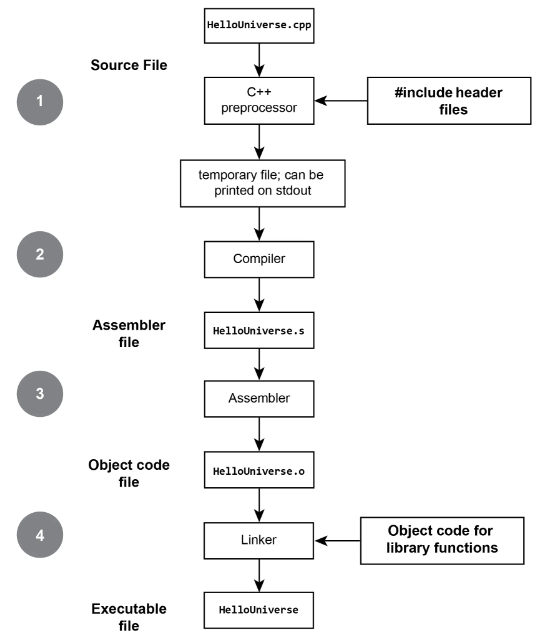
\includegraphics[width=0.5\textwidth]{p241.png}
		\caption{C++ compilation}
		\label{fig:p241}
	\end{figure}

\end{question}











